\chapter{Teori og tidligere arbeid}
\label{kap:teori}
I dette kapittelet beskrives utvalget av faglitteratur som vi baserer oss på i dette prosjektet. Det beskrives hvorfor de ble valgt og hvordan vi fant frem til disse. I tillegg beskrives teorien i dypere detalj, og litt om historien bak metoden. 

\section{Utvalg av faglitteratur}
Rotårsaksanalyse som helhet finnes det mye litteratur om, men metodene er veldig spredt. Innen informasjonsikkerhet finnes det lite bruk av rotårsaksanlayse. Vi har valgt boken ``Root Cause Analysis: Simplified Tools and Techniques'' av Fagerhaug og Andersen \cite{RCA} som gir en generell beskrivelse av rotårsaksmetodikken, men ikke spesifikt for informasjonssikkerhet. Vi har i tillegg brukt en bacheloroppgave fra 2016 \cite{RCARapport} som så på anvendelsen av rotårsaksanalyse innen informasjonssikkerhet.

\subsection{Hvorfor ble disse valgt?}
Vi valgte boken \cite{RCA} på anbefaling av oppdragsgiver og fordi vi ville se hvor godt den fungerte innen informasjonssikkerhet. Forfatterne av boken \cite{RCA} har i stor grad fokusert på de menneskelige årsakene og i mindre grad på tekniske årsaker. Vi ville se hvor godt denne tilnærmingen fungerer i informasjonsikkerhet, der de fleste problemer er menneskeskapt. Vi vil spesielt se hvor godt boka fungerte som en samlet metodikk for rotårsaksanalyse innen informasjonsikkerhet. Bacheloroppgaven \cite{RCARapport} ble valgt da den er en av få studier som systematisk tar for seg rotårsaksanalyse i informasjonssikkerhetssammenheng. 

\section{Teori}
Rotårsaksanalyse er en fremgangsmåte for å finne roten til et problem og eliminere det. RCA analyserer de underliggende faktorene og bruker årsakene til å finne roten til problemet. RCA er en reaktiv prosess som finner svar på problemer basert på skjulte årsaker og deres effekt, istedenfor å undersøke den mest åpenbare årsaken. Dette gjør at RCA er ofte komplekst og tidkrevende, men når rotårsaken først er funnet kan løsningene fjerne problemet helt. 

\subsection{Historie}
Det har finnes flere varianter av rotåsaksanalyse opp gjennom tidene, men mannen som er kreditert med å finne opp rotårsaksanalyse er grunnleggeren av Toyota, Sakichi Toyoda. Hans versjon av RCA ble tatt i bruk av Toyota produksjonsprosess i 1958 og ble kalt ``5 Whys''. Som tidligere sagt har RCA forandret seg over tidene for å imøtekomme de forskjellige feltene. Nå brukes RCA som verktøy i flere felter som transport, medisin og luftfart \cite{Teori}. 
    
\subsection{Ulike nivåer av årsaker}
Et problem er som regel ikke et resultat av en årsak, men heller en kombinasjon av flere årsaker på flere forskjellige nivåer. Dette vil si at årsaker påvirker andre årsaker helt opp til det synlige problemet. Årsaker defineres i tre forskjellige grupper: 

\begin{description}
    \item[Symptomer] er ikke å regne som faktiske årsaker, men heller bevis på eksisterende problemer.
    \item[Første-nivå årsak] er årsåker som leder direkte til et problem.
    \item[Høy-nivå årsaker] er årsåker som blir til første-nivå årsaker. Selv om de ikke direkte er årsak til problemmet, skaper høy-nivå årsak lenker i kjeden av årsak-virkningsforholdet som til slutt fører til problemet. Den høyeste nivå årsaken er rotårsaken.  
\end{description}
Noen problemer har flere årsaker som er forbundet av de forskjellige faktorer som kombinert blir til problemet.

\begin{figure}[H]
    \centering
    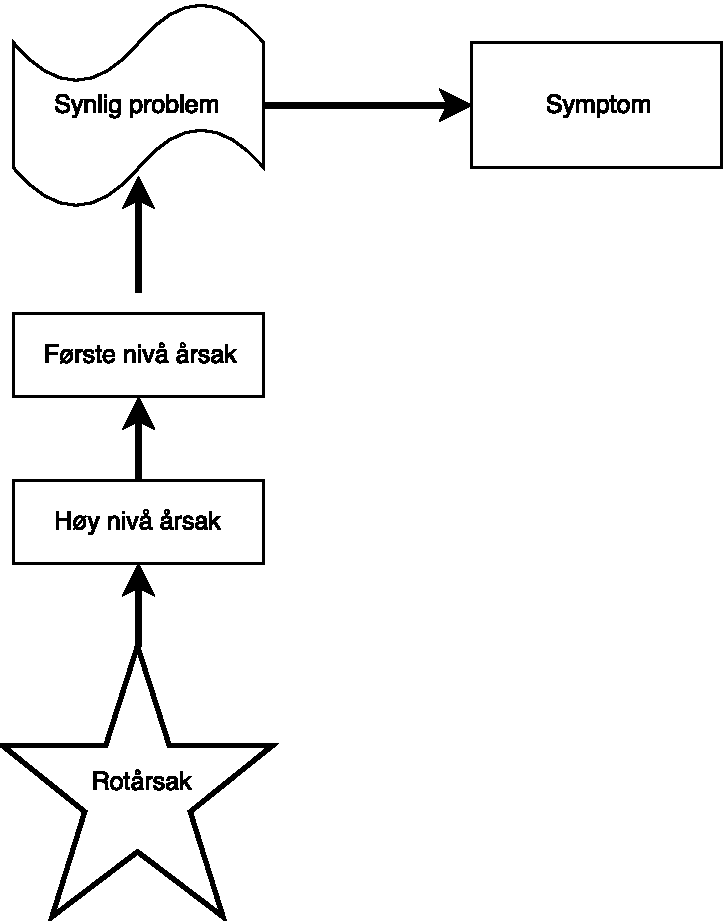
\includegraphics[scale=0.6]{main/bilder/nivaa.pdf}
    \caption[Nivåer av årsaker]{De forskjellige nivåer til problemet}
    \label{fig:nivaa}
\end{figure}

Vi ser fra figuren at rotårsaken er det som setter i gang årsak-virkningskjeden som leder til det synlige problemet. 

\subsection{Root Cause Analysis: Simplified tools and techniques}
Denne boken er andre utgave og bygger mer på hele problemet enn første utgaven. Der første utgaven stoppet etter å identifisert rotårsaken, gir andre utgave deg verktøy til å komme helt til løsningsimplenteringen. Den gjør det igjennom å strukturer analysen i 7 steg i en typisk fossefallmetodikk. Boken har i tillegg to ekstra kapittel der den tar for seg eksempelcaser og retningslinjer for verktøyvalg i form av et flytdiagram. 

\subsection{Tidligere arbeid innen informasjonssikkerhet}
I 2016 ga NTNU en bacheloroppgave som heter ``Bruk av rotårsaksanalyse i informasjonssikkerhet''\cite{RCARapport}. Oppgaven ser på hvor godt rotårsaksanalyse fungerer i informasjonsikkerhet. For å finne det ut gikk de igjennom rotårsaksanalyse på tre caser. Konklusjonene de kom frem til var at de fikk tilstrekkelig svar på sine forskningspørsmål. For våres del er de viktigste konklusjonene til deres rapport\cite{RCARapport} at de fant ut: ved bruk av rotårsaksanalyse var det mulig å komme frem til problemsituasjoner som ikke var synlig ved bruk av andre verktøy i informasjonssikkerhet.  

\subsection{Rotårsaksanalyse sammenlignet med risikoanalyse}
En risikoanalyse ser på sannsynligheten for at en trussel kan skje og mulige konsekvenser av dette. Risikoen regnes ut fra sannsynlighet og konsekvens, samt eksisterende kontroller. I risikoanalysen vil dataene brukes til å finne mulige preventive og reaktive tiltak som kan føre riskoen ned på et akseptabelt nivå. Rotårsaksanalyse vil på sin side gjøre en systematisk gjenomgang for å finne de underliggende årsakene til feil eller svikt. En rotårsaksanalyse gjøres etter et problem har oppstått, i motsetning til riskoanalyse som gjøres for å behandle fremtidige situasjoner. 